\chapter{Implementacija i korisničko sučelje}
		
		
		\section{Korištene tehnologije i alati}
			 		
			Komunikacija unutar tima ostvaruje se korištenjem popularnih aplikacija, kao što su \textbf{WhatsApp}$^{[1]}$ i \textbf{Discord}$^{[2]}$. Za modeliranje UML dijagrama koristili smo \textbf{Astah UML}$^{[3]}$.
			
			\textbf{Git}$^{[4]}$ je centralni sustav za upravljanje izvornim kodom, a projektni udaljeni repozitorij dostupan je na web platformi \textbf{GitHub}$^{[5]}$.
			
			Razvoj frontend-a izveden je u \textbf{JavaScriptu}$^{[6]}$ koristeći biblioteku \textbf{React}$^{[7]}$ koja je održavana od strane Facebooka. Za uređivanje koda koristili smo Microsftov uređivač koda \textbf{Visual Studio Code (VSCode)}$^{[8]}$, koji pruža izvrsnu podršku za razvoj modernih web aplikacija.
			
			Za backend, koristili smo \textbf{IntelliJ IDEA}$^{[9]}$, integrirano razvojno okruženje (IDE) tvrtke JetBrains. IntelliJ pruža snažnu potporu za razvoj Java Spring aplikacija.
			
			Baza podataka koju koristimo je \textbf{PostgreSQL}$^{[10]}$. PostgreSQL je snažan open-source sustav za upravljanje bazama podataka.
			
			Pogon aplikacije vršimo putem \textbf{Render}$^{[11]}$ platforme, koja omogućava jednostavan i efikasan proces. Render pruža usluge poput web hostinga, skaliranja aplikacija i upravljanja resursima u oblaku.
			
			Za dokumentaciju koristimo \textbf{TeXstudio}$^{[12]}$ koji podržava LaTeX. LaTeX je sistem za pripremu dokumenata koji se koristi za visokokvalitetno formatiranje tekstova.
			
			$^{1}$\url{https://www.whatsapp.com/}
			
			$^{2}$\url{https://discord.com/}
			
			$^{3}$\url{https://astah.net/products/astah-uml/}
			
			$^{4}$\url{https://git-scm.com/}
			
			$^{5}$\url{https://github.com/}
			
			$^{6}$\url{https://www.javascript.com/}
			
			$^{7}$\url{https://reactjs.org/}
			
			$^{8}$\url{https://code.visualstudio.com/}
			
			$^{9}$\url{https://www.jetbrains.com/idea/}
			
			$^{10}$\url{https://www.postgresql.org/}
			
			$^{11}$\url{https://render.com/}
			
			$^{12}$\url{https://www.texstudio.org/}
			
			\eject 
		
	
		\section{Ispitivanje programskog rješenja}
			
			\textbf{\textit{dio 2. revizije}}\\
			
			 \textit{U ovom poglavlju je potrebno opisati provedbu ispitivanja implementiranih funkcionalnosti na razini komponenti i na razini cijelog sustava s prikazom odabranih ispitnih slučajeva. Studenti trebaju ispitati temeljnu funkcionalnost i rubne uvjete.}
	
			
			\subsection{Ispitivanje komponenti}
			\textit{Potrebno je provesti ispitivanje jedinica (engl. unit testing) nad razredima koji implementiraju temeljne funkcionalnosti. Razraditi \textbf{minimalno 6 ispitnih slučajeva} u kojima će se ispitati redovni slučajevi, rubni uvjeti te izazivanje pogreške (engl. exception throwing). Poželjno je stvoriti i ispitni slučaj koji koristi funkcionalnosti koje nisu implementirane. Potrebno je priložiti izvorni kôd svih ispitnih slučajeva te prikaz rezultata izvođenja ispita u razvojnom okruženju (prolaz/pad ispita). }
			
			
			
			\subsection{Ispitivanje sustava}
			
			 \textit{Potrebno je provesti i opisati ispitivanje sustava koristeći radni okvir Selenium\footnote{\url{https://www.seleniumhq.org/}}. Razraditi \textbf{minimalno 4 ispitna slučaja} u kojima će se ispitati redovni slučajevi, rubni uvjeti te poziv funkcionalnosti koja nije implementirana/izaziva pogrešku kako bi se vidjelo na koji način sustav reagira kada nešto nije u potpunosti ostvareno. Ispitni slučaj se treba sastojati od ulaza (npr. korisničko ime i lozinka), očekivanog izlaza ili rezultata, koraka ispitivanja i dobivenog izlaza ili rezultata.\\ }
			 
			 \textit{Izradu ispitnih slučajeva pomoću radnog okvira Selenium moguće je provesti pomoću jednog od sljedeća dva alata:}
			 \begin{itemize}
			 	\item \textit{dodatak za preglednik \textbf{Selenium IDE} - snimanje korisnikovih akcija radi automatskog ponavljanja ispita	}
			 	\item \textit{\textbf{Selenium WebDriver} - podrška za pisanje ispita u jezicima Java, C\#, PHP koristeći posebno programsko sučelje.}
			 \end{itemize}
		 	\textit{Detalji o korištenju alata Selenium bit će prikazani na posebnom predavanju tijekom semestra.}
			
			\eject 
		
		
		\section{Dijagram razmještaja}
			
			
			 Slika \ref{fig:DijRazm} prikazuje odnos komponenti u sustavu. Klijent preko svog Korisničkog uređaja putem Web preglednika pirstupa Poslužitelju putem HTTP protokola. Poslužitelj se sastoji od Web apliakcije koja izvlači podatke iz baze podataka te zato ovisi o njoj.
			 
			 \begin{figure}[H]
			 	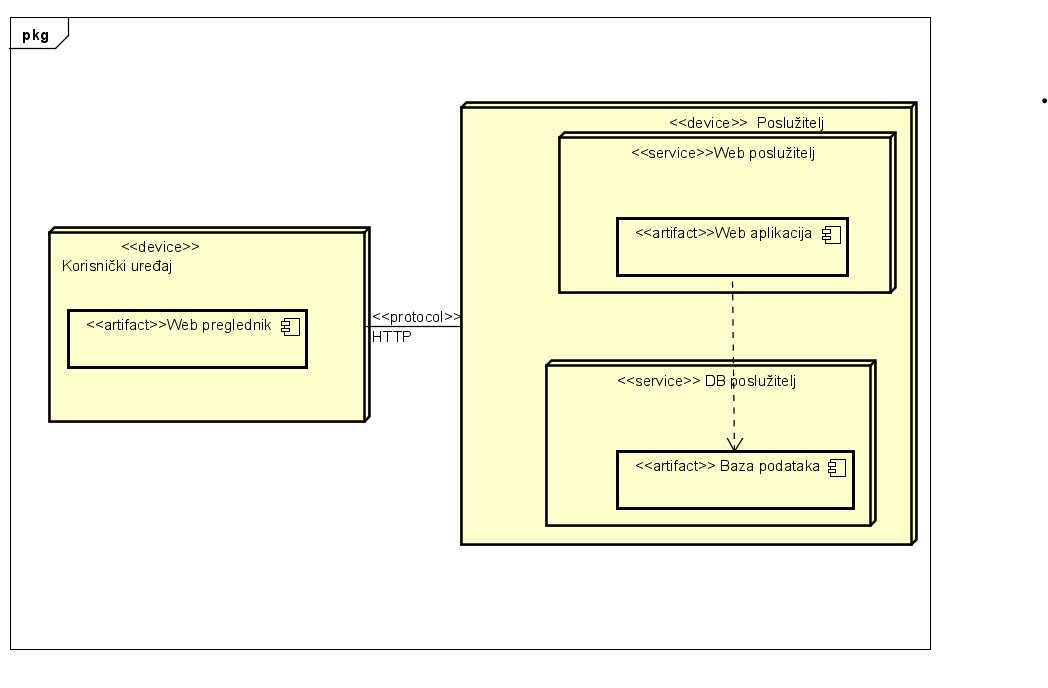
\includegraphics[scale=0.4]{slike/dijagramRaz.jpeg} %veličina slike u odnosu na originalnu datoteku i pozicija slike
			 	\centering
			 	\caption{Dijagram Razmještaja}
			 	\label{fig:DijRazm}
			 \end{figure}
			
			\eject 
		
		\section{Upute za puštanje u pogon}
		
			\textbf{\textit{dio 2. revizije}}\\
		
			 \textit{U ovom poglavlju potrebno je dati upute za puštanje u pogon (engl. deployment) ostvarene aplikacije. Na primjer, za web aplikacije, opisati postupak kojim se od izvornog kôda dolazi do potpuno postavljene baze podataka i poslužitelja koji odgovara na upite korisnika. Za mobilnu aplikaciju, postupak kojim se aplikacija izgradi, te postavi na neku od trgovina. Za stolnu (engl. desktop) aplikaciju, postupak kojim se aplikacija instalira na računalo. Ukoliko mobilne i stolne aplikacije komuniciraju s poslužiteljem i/ili bazom podataka, opisati i postupak njihovog postavljanja. Pri izradi uputa preporučuje se \textbf{naglasiti korake instalacije uporabom natuknica} te koristiti što je više moguće \textbf{slike ekrana} (engl. screenshots) kako bi upute bile jasne i jednostavne za slijediti.}
			
			
			 \textit{Dovršenu aplikaciju potrebno je pokrenuti na javno dostupnom poslužitelju. Studentima se preporuča korištenje neke od sljedećih besplatnih usluga: \href{https://aws.amazon.com/}{Amazon AWS}, \href{https://azure.microsoft.com/en-us/}{Microsoft Azure} ili \href{https://www.heroku.com/}{Heroku}. Mobilne aplikacije trebaju biti objavljene na F-Droid, Google Play ili Amazon App trgovini.}
			
			
			\eject 